%%%%%%%%%%%%%%%%%%%%%%%%%%%%%%%%%%%%%%%%%%%%%%%%%%%%%%%%%%%%%%%%%%%%%%%%%%%

\documentclass{standalone}

\usepackage{amsmath}
\usepackage{mathptmx}
\usepackage{pgfplots}
\usetikzlibrary{external}
\tikzexternalize{sunflower-regression}
\pgfplotsset{compat=1.16}

%% IEEE uses Times Roman font, so we'll default to Times.
%% These three commands make up the entire times.sty package.
\renewcommand{\rmdefault}{ptm}
\renewcommand{\ttdefault}{pcr}
\normalfont\selectfont

\begin{document}

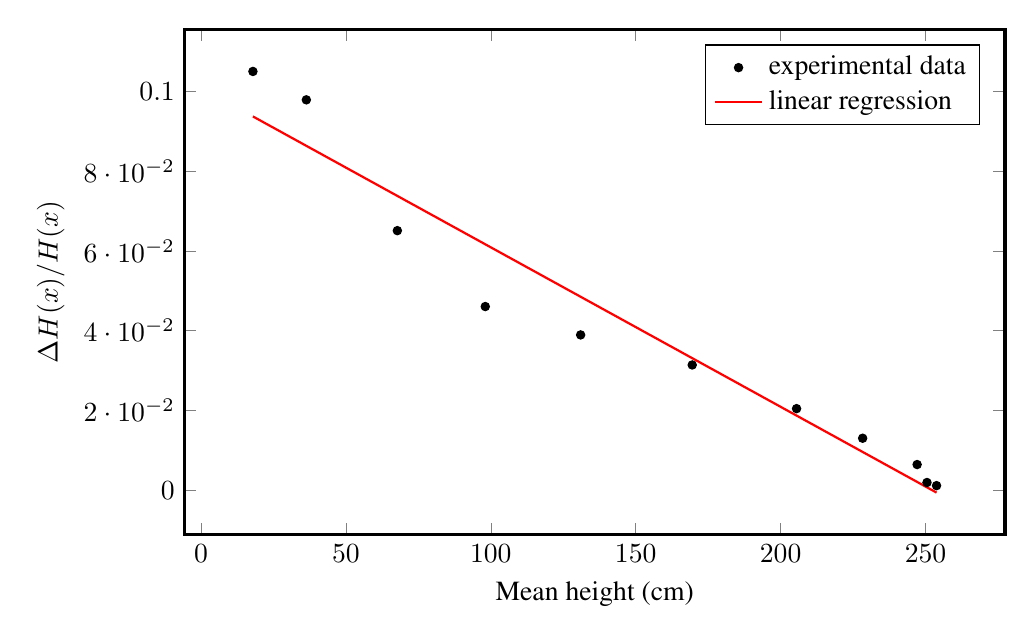
\begin{tikzpicture}
\tikzset{%%
  every mark/.append style={scale=1.0},%%
  scale=1.0%%
}
\pgfplotsset{%%
  every axis/.append style={font=\normalsize}%%
}
%%
\begin{axis}[%%
  axis line style=very thick,%%
  dotStyle/.style={mark size=1.5,black,mark color=black,mark=*,only marks},%%
  enlargelimits=true,%%
  height=8cm,%%
  legend cell align=left,%%
  legend pos=north east,%%
  plotStyle/.style={%%
    domain=17.93:253.8,%%
    mark=none,%%
    smooth,%%
    thick%%
  },%%
  width=12cm,%%
  %% x axis
  xlabel={\normalsize Mean height~(cm)},%%
  %% y axis
  ylabel={\normalsize $\Delta H(x) / H(x)$}%%
]
%%
%%
\addplot[dotStyle] coordinates {
  (17.93, 0.105011552864314)
  (36.36, 0.097890146157473)
  (67.76, 0.065082644628099)
  (98.1, 0.04604630843163)
  (131, 0.038931297709924)
  (169.5, 0.031394858828487)
  (205.5, 0.02043795620438)
  (228.3, 0.013015455853827)
  (247.1, 0.006417297797306)
  (250.5, 0.001910464784716)
  (253.8, 0.001125745806597)
};
\addlegendentry{experimental data}
%%
%%
\addplot+ [plotStyle,red]
{-0.0004*x + 0.1009};
\addlegendentry{linear regression}
\end{axis}
\end{tikzpicture}

\end{document}
